%==========================================================
\section{Exercise 1}\label{sec:ex1}
%==========================================================
In Figure \ref{fig:ex36-1} and \ref{fig:ex36-2} I show that
\begin{align*}
    \mathbf{\beta}_{Ridge} &= \big( \mathbf{X}^{T} \mathbf{X} + \lambda \mathbf{I} \big)^{-1} \mathbf{X}^{T} \mathbf{y}
\end{align*}

\begin{figure}[h!]
    \centering
    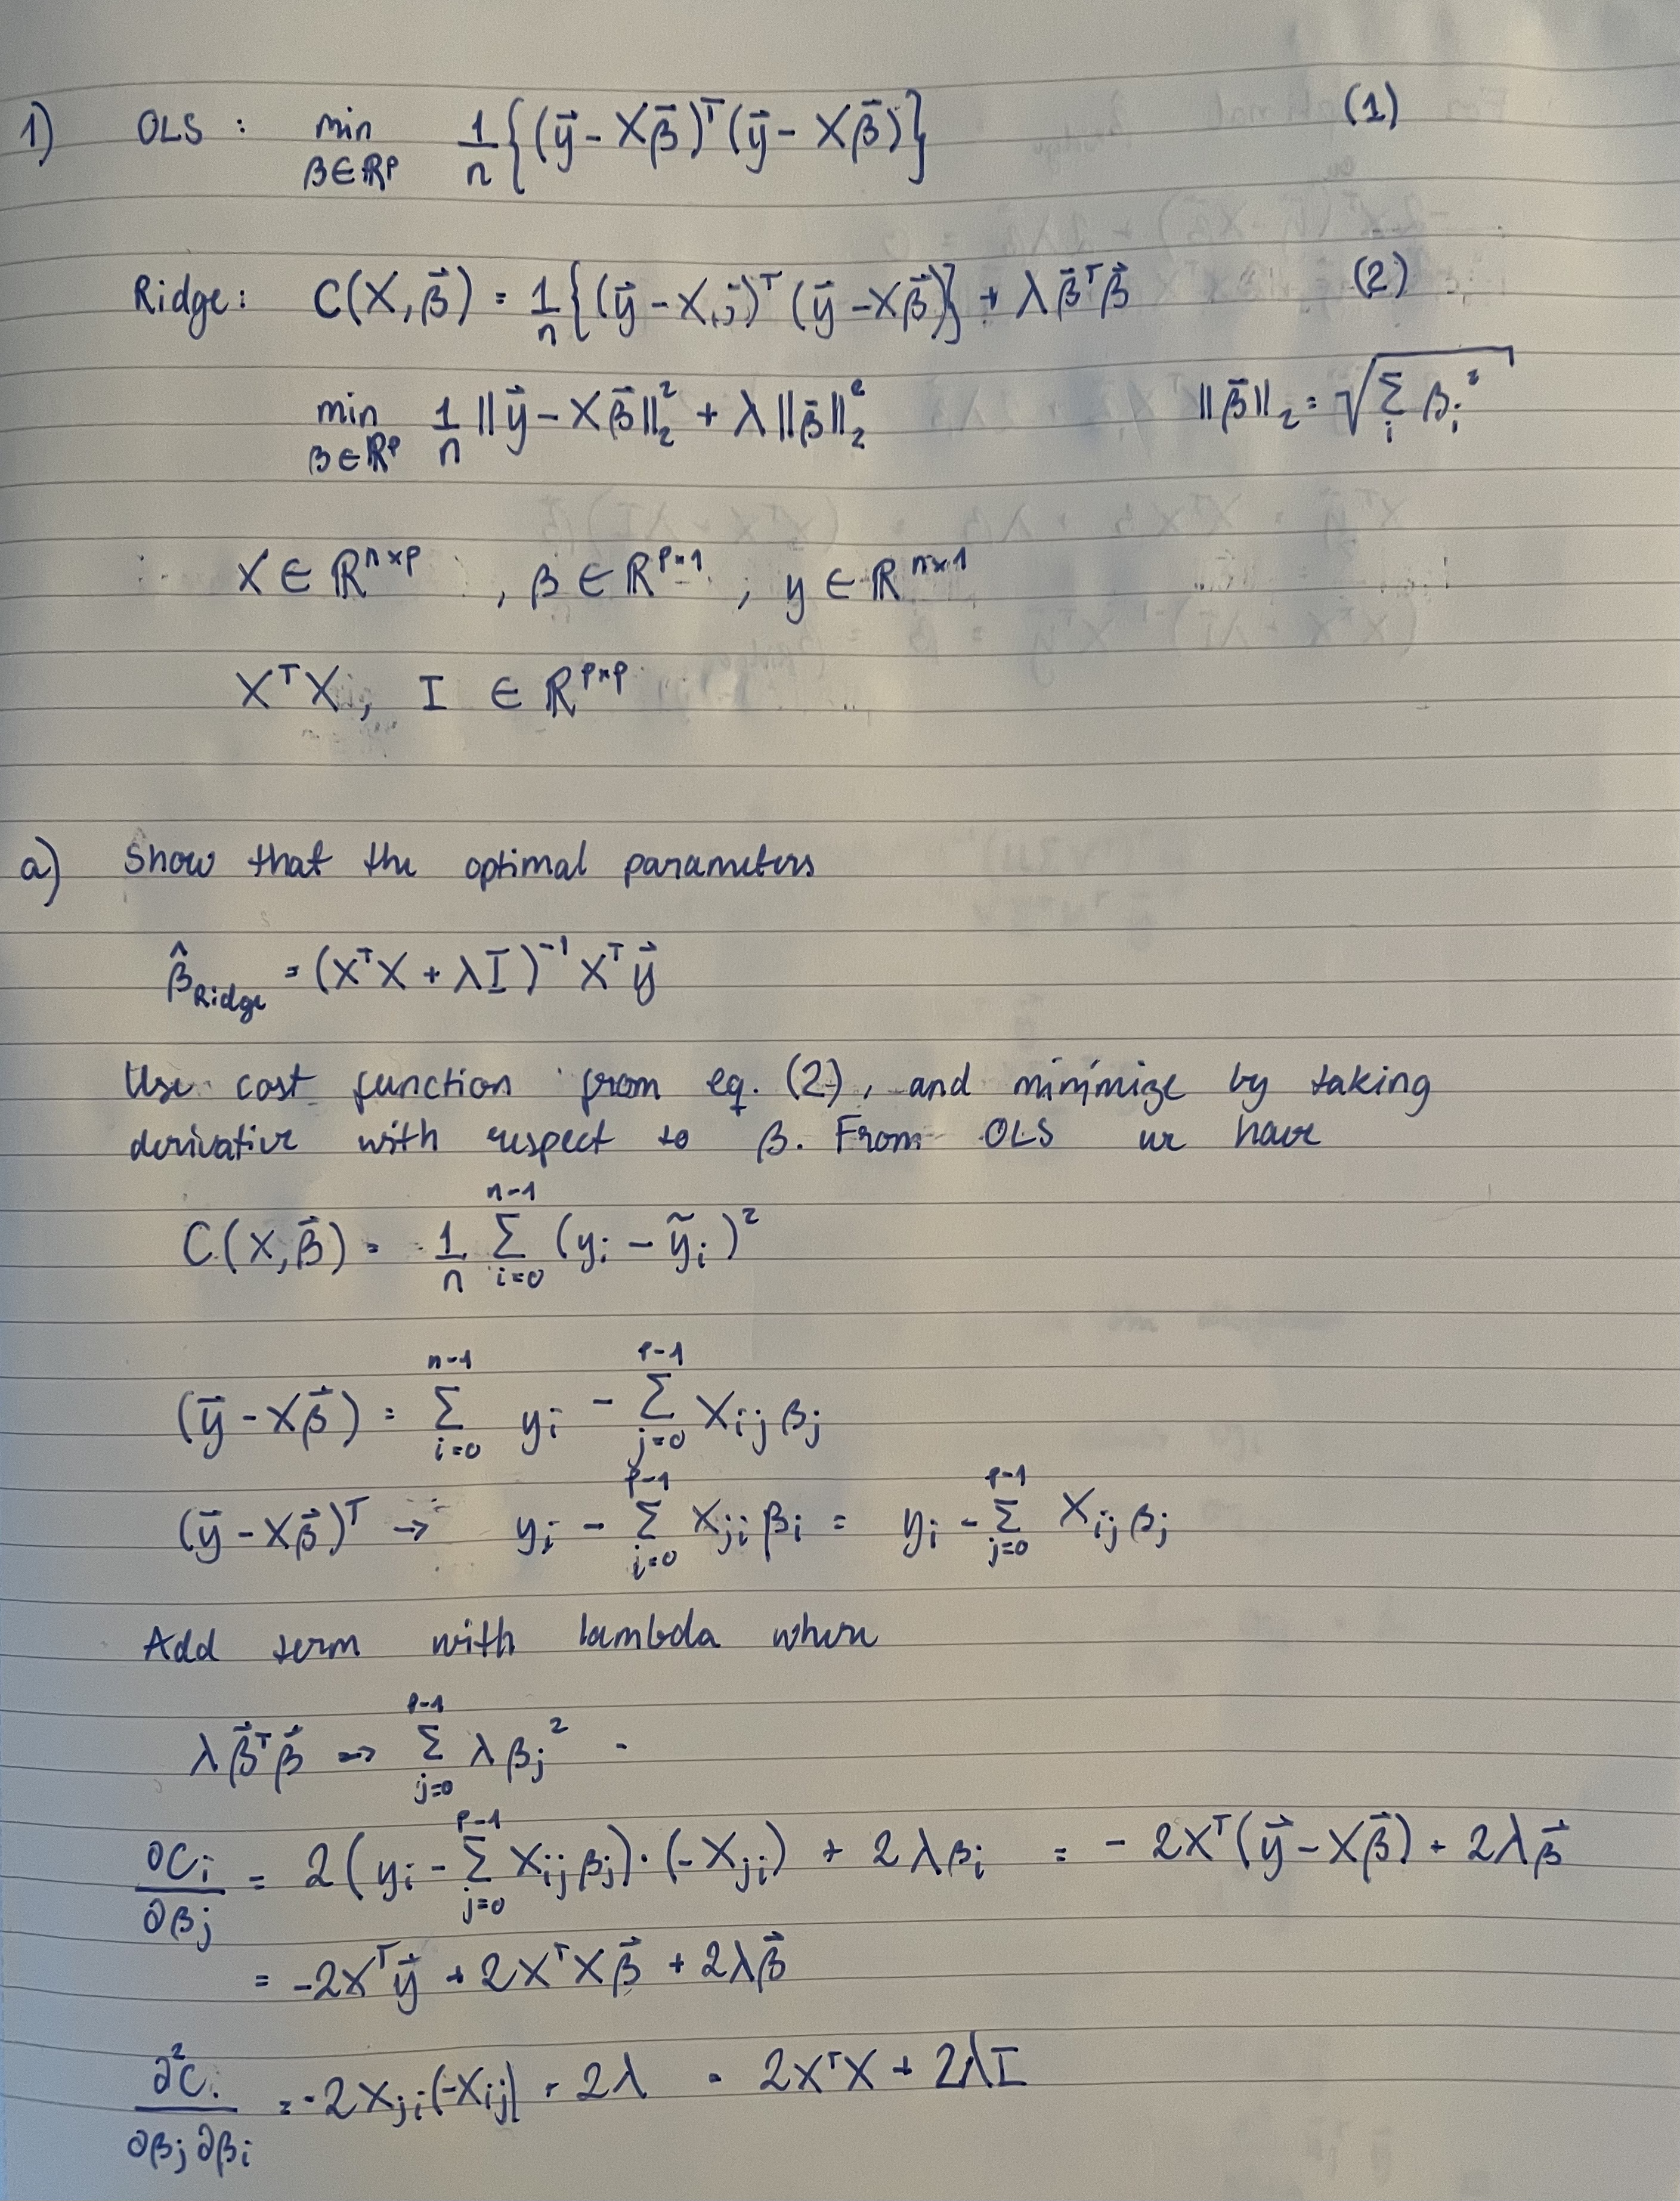
\includegraphics[width=0.7\linewidth]{latex/figures/ex36-1.jpeg}
    \caption{Exercise 1a}
    \label{fig:ex36-1}
\end{figure}

\begin{figure}[h!]
    \centering
    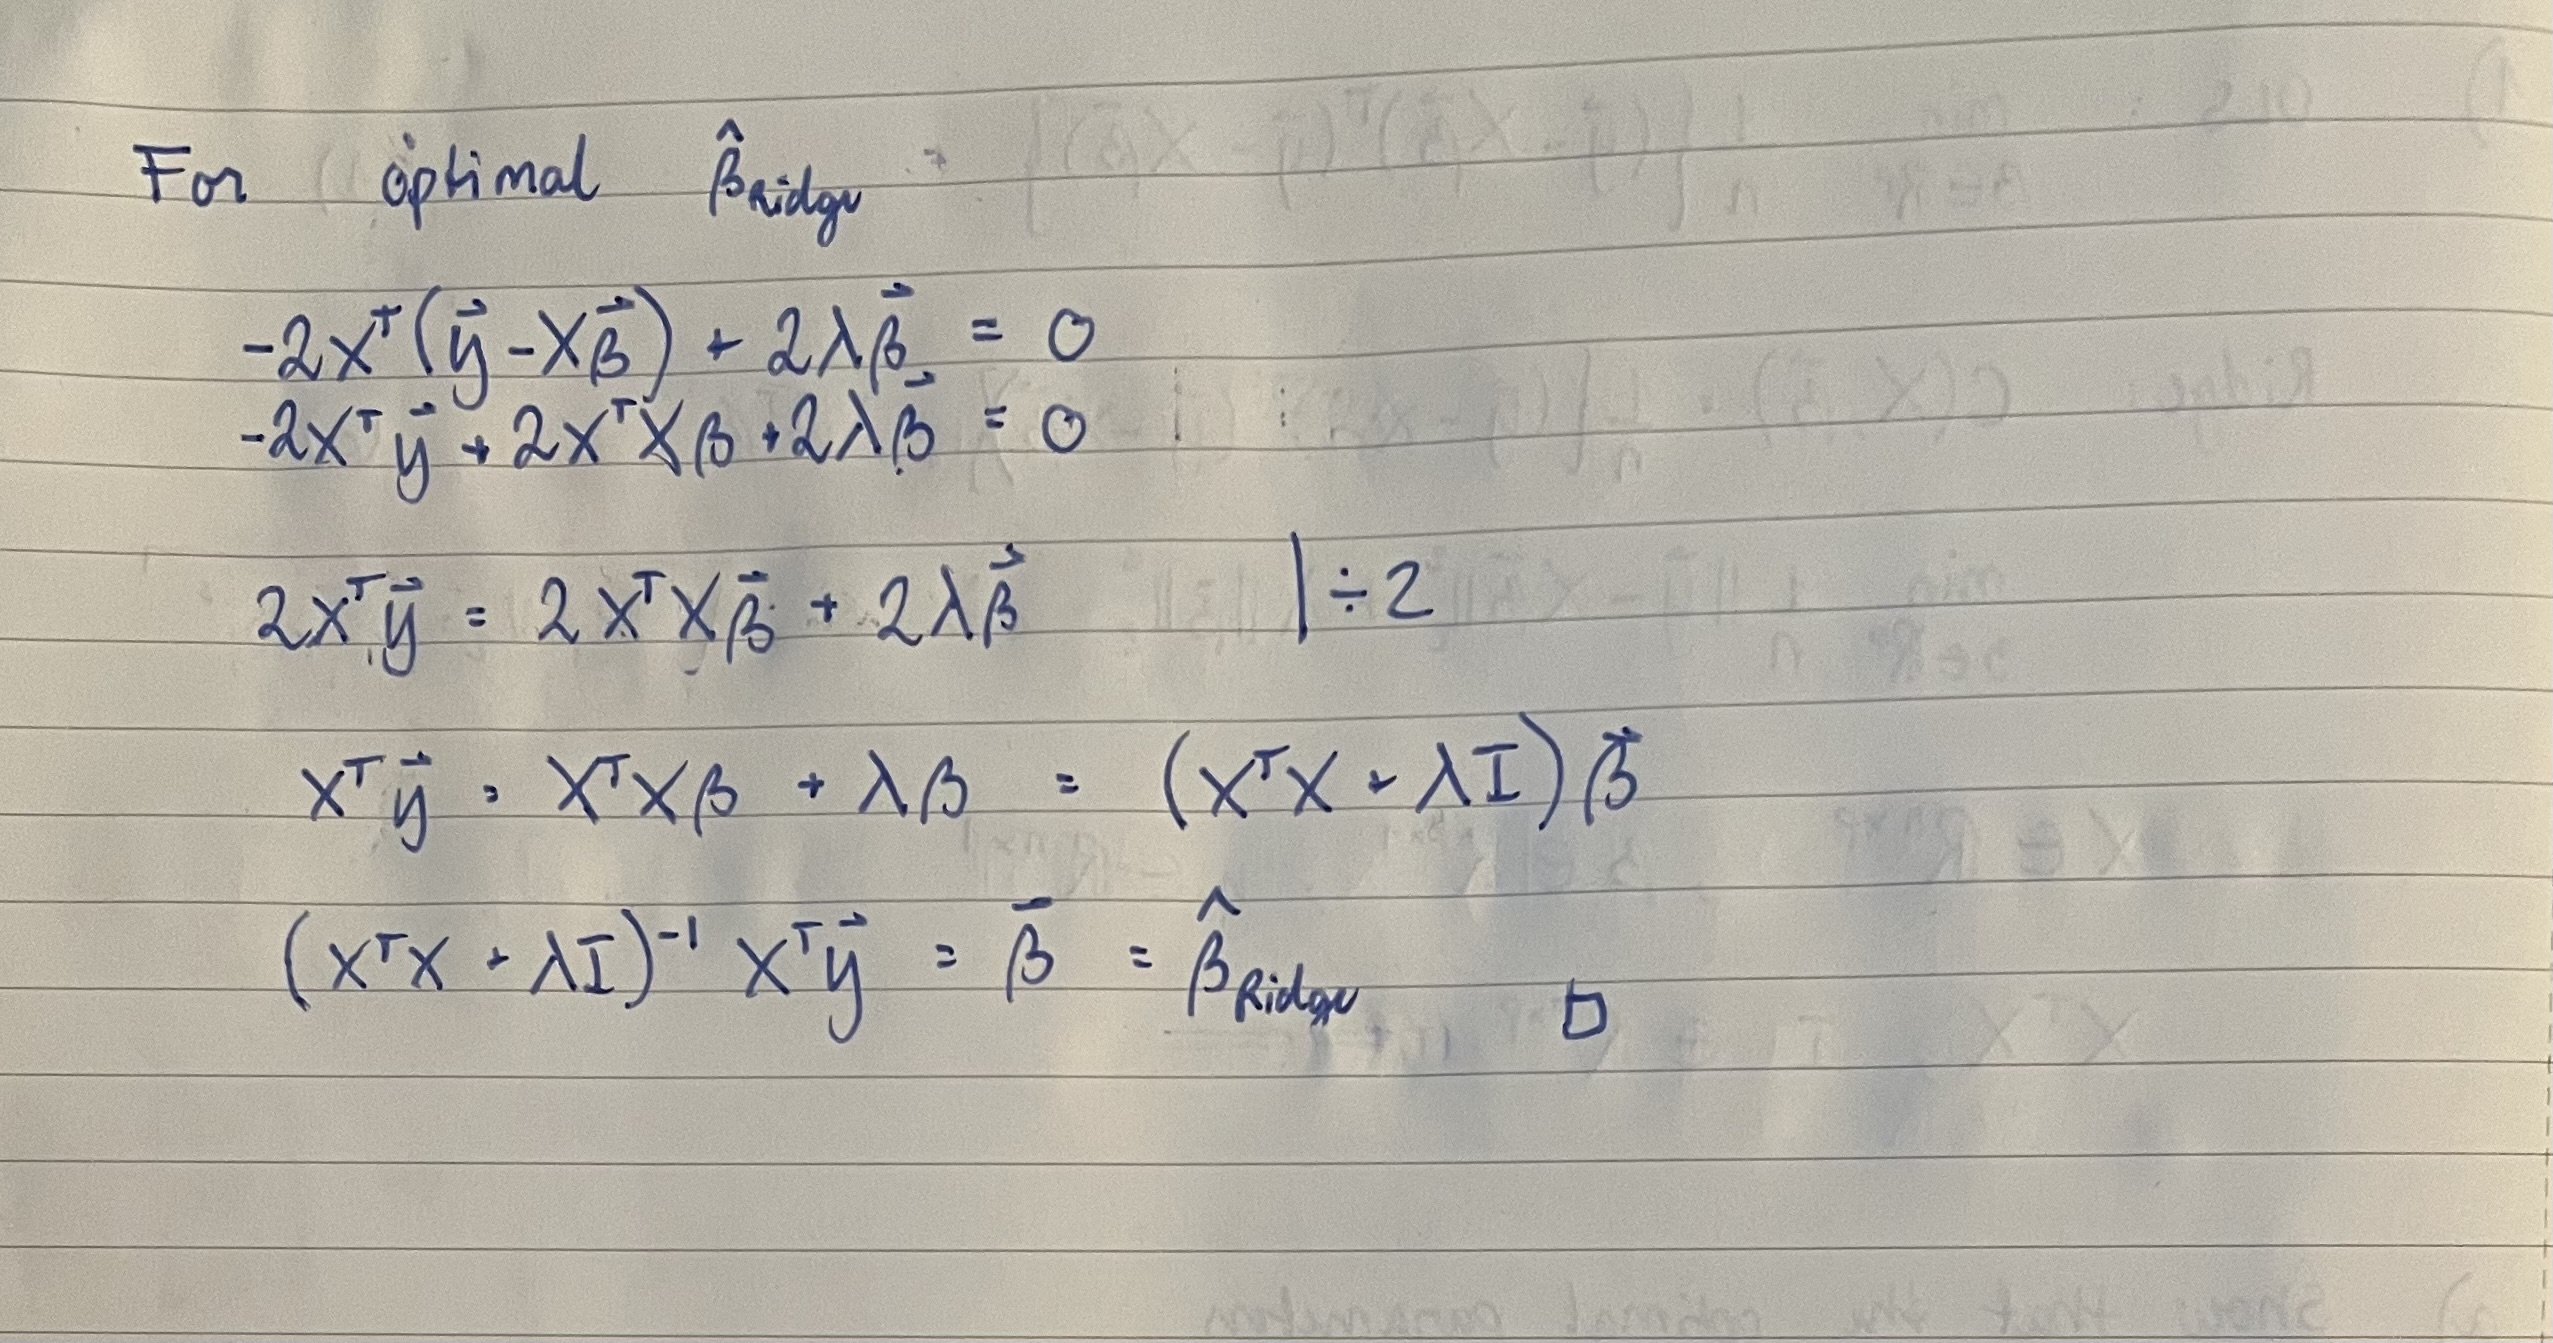
\includegraphics[width=0.7\linewidth]{latex/figures/ex36-2.jpeg}
    \caption{Cont. exercise 1a}
    \label{fig:ex36-2}
\end{figure}

And in Figure \ref{fig:ex36-3} I show that 
\begin{align*}
    \mathbf{\beta}_{OLS} &= \big( \mathbf{X}^{T} \mathbf{X} \big)^{-1} \mathbf{X}^{T} \mathbf{y}
\end{align*}

\begin{figure}[h!]
    \centering
    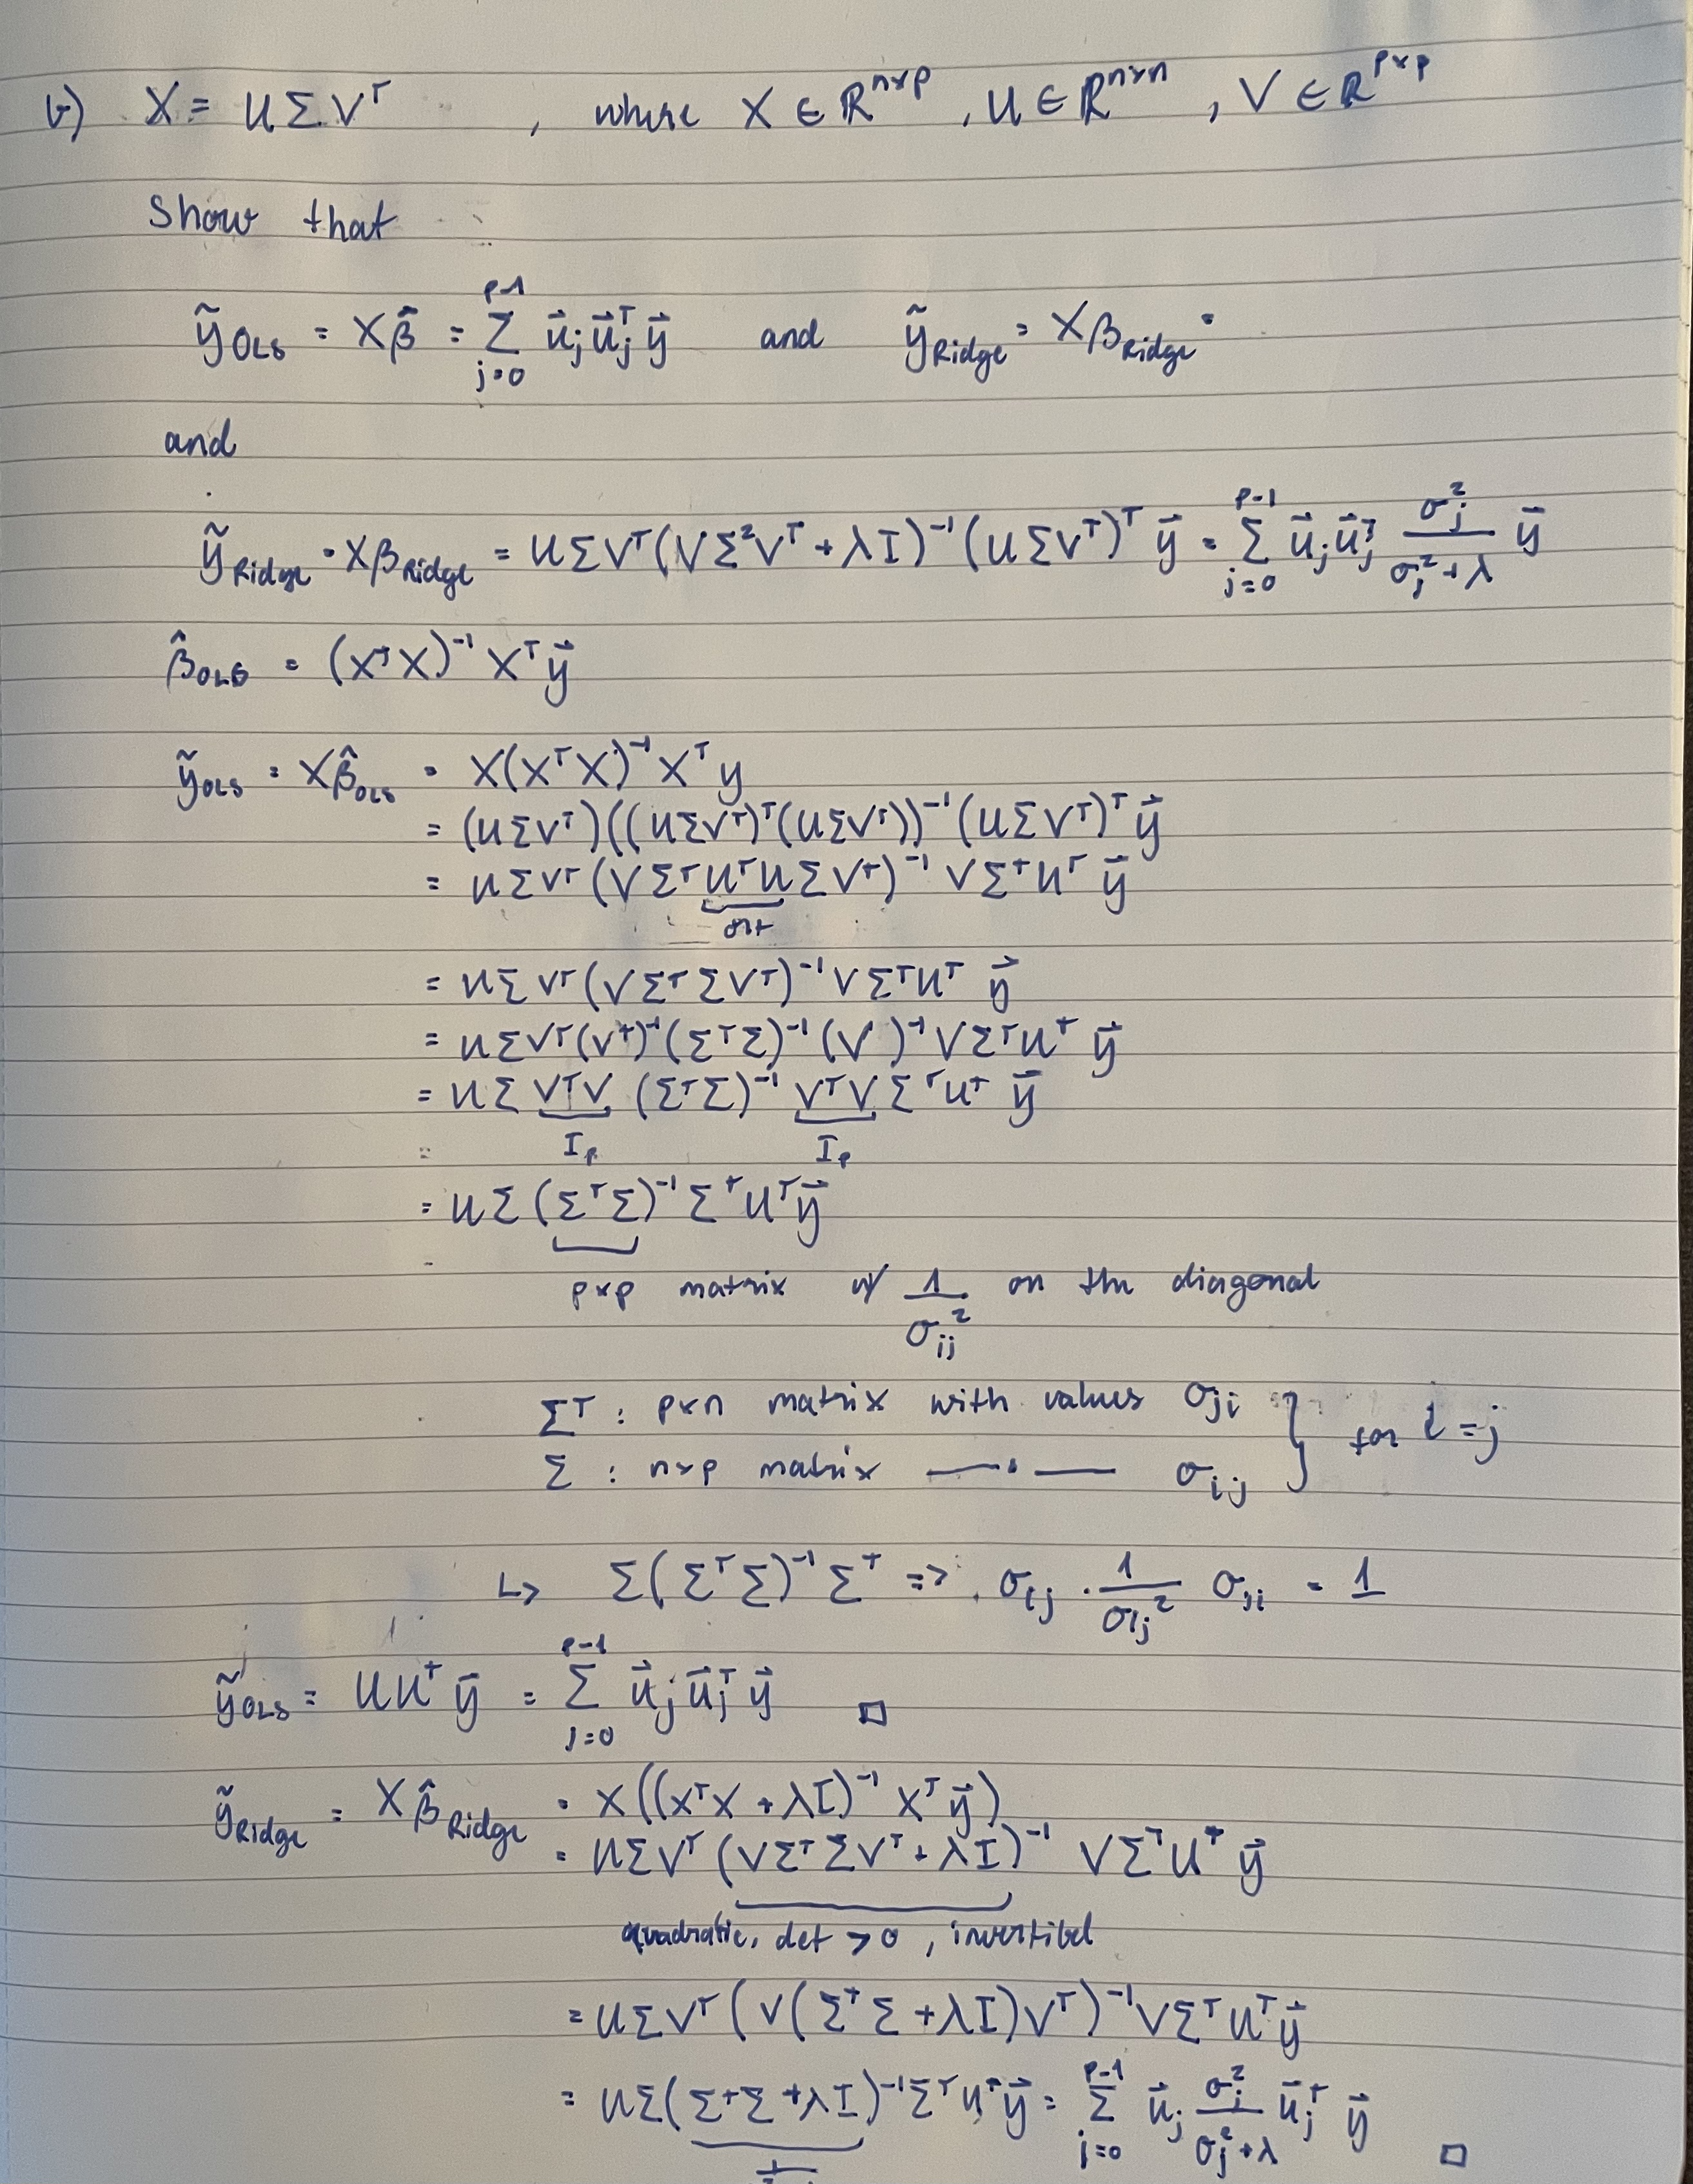
\includegraphics[width=0.7\linewidth]{latex/figures/ex36-3.jpeg}
    \caption{Exercise 1b}
    \label{fig:ex36-3}
\end{figure}

%==========================================================
\section{Exercise 2}\label{sec:ex2}
%==========================================================
\begin{figure}

\begin{lstlisting}[language=Python]
class Regression:
    def __init__(self, degree, lmbda=None) -> None:
        self._degree = degree + 1
        self._lmbda = lmbda

    def fit_ols(self, X_train, y_train):
        X_T = X_train.T
        XTX = X_T @ X_train
        self._beta = np.linalg.pinv(XTX) @ X_T @ y_train 

    def fit_ridge(self, X_train, y_train):
        X_T = X_train.T
        XTX = X_T @ X_train
        self._beta = np.linalg.pinv(XTX + self._lmbda*np.eye(len(XTX))) @ X_T @ y_train 
    
    def predict(self, X_test):
        y_pred = X_test @ self._beta
        return y_pred 
    

def evaluate_models():
    n = 100
    p = [5, 10, 15]
    lmbdas = [0.0001, 0.001, 0.01, 0.1, 1.0]

    x = np.random.rand(n)
    y = 2.0 + 5*x**2 + 0.1*np.random.randn(n)

    mse_train = np.zeros((len(p), len(lmbdas)+1))
    mse_test = np.zeros((len(p), len(lmbdas)+1))

    for i, degree in enumerate(p):
        X = design_matrix(x, degree)
        # Add scaling in design matrix function
        # X_scaled = X - X.mean(axis=0)

        # X_train, X_test, y_train, y_test = train_test_split(X_scaled, y, test_size=0.2)
        X_train, X_test, y_train, y_test = train_test_split(X, y, test_size=0.2)
        X_train_mean = np.mean(X_train, axis=0)
        y_train_mean = np.mean(y_train)

        X_train = X_train - X_train_mean
        y_train = y_train - y_train_mean


        model_ols = Regression(degree)
        model_ols.fit_ols(X_train, y_train)
        y_ols_train = model_ols.predict(X_train)
        mse_train[i, 0] = mean_squared_error(y_train, y_ols_train)
        y_ols_test = model_ols.predict(X_test-X_train_mean)
        mse_test[i, 0] = mean_squared_error(y_test, y_ols_test+y_train_mean)

        for j, lmbda in enumerate(lmbdas):
            model_ridge = Regression(degree, lmbda)
            model_ridge.fit_ridge(X_train, y_train)
            y_ridge_train = model_ridge.predict(X_train)
            mse_train[i, j+1] = mean_squared_error(y_train, y_ridge_train)
            y_ridge_test = model_ridge.predict(X_test-X_train_mean)
            mse_test[i, j+1] = mean_squared_error(y_test, y_ridge_test+y_train_mean)

    fig, (ax1, ax2) = plt.subplots(1, 2, figsize=(12, 6))
    train_mse = mse_train.T
    test_mse = mse_test.T
    labels = [
        "OLS", 
        fr"Ridge, $\lambda$ = {lmbdas[0]}",
        fr"Ridge, $\lambda$ = {lmbdas[1]}",
        fr"Ridge, $\lambda$ = {lmbdas[2]}",
        fr"Ridge, $\lambda$ = {lmbdas[3]}",
        fr"Ridge, $\lambda$ = {lmbdas[4]}"]

    for i in range(len(lmbdas)+1):
        ax1.plot(p, train_mse[i], label=labels[i])
        ax2.plot(p, test_mse[i], label=labels[i])

    ax1.legend()
    ax1.set_title("Train")
    ax1.set_xlabel("Polynomial degree")
    ax1.set_ylabel("MSE")
    ax2.legend()
    ax2.set_title("Test")
    ax2.set_xlabel("Polynomial degree")
    # fig.savefig("../latex/figures/week36_ex2.pdf")
    plt.show()


if __name__ == '__main__':
    np.random.seed(2024)
    evaluate_models()
\end{lstlisting}
\end{figure}